\documentclass[nofootinbib,aps]{revtex4}

\usepackage{amsmath,amssymb,graphicx,color,microtype}
\usepackage{listings}
\usepackage{xcolor}
\usepackage{framed,subfigure,csvsimple}
\definecolor{myorange}{RGB}{255,165,0}
\definecolor{darkgreen}{RGB}{0,120,0}

\lstnewenvironment{pythoncode}[1][]
{
    \lstset{
        language=Python,
        basicstyle=\small\ttfamily,
        keywordstyle=\color{blue},
        stringstyle=\color{myorange},
        commentstyle=\color{darkgreen},
        numbers=left,
        framexleftmargin=5mm,
        numberstyle=\tiny\color{gray},
        numbersep=-2pt,
        breaklines=true,
        captionpos=t,
        language=python,
        #1 % Additional options
    }
}
{}


\begin{document}

\title{Python Final Project for analysis of Light Curve}
\date{\today}
\author{Lingyu Xia\\ID Number: EJ7410069}


\maketitle

\section{Code-Main.py}


\begin{framed}
\begin{pythoncode}[caption={main.py code}]
    import pandas as pd
    import numpy as np
    import matplotlib.pyplot as plt
    from scipy.stats import norm
    from statsmodels.graphics.tsaplots import plot_acf
    from statsmodels.tsa.seasonal import seasonal_decompose
    from scipy.interpolate import interp1d
    import logging


    ######### BASE CLASS ##############

    class TimeSeriesAnalyzer:
    def __init__(self, filename, energy_range, title):
        self.filename = filename
        self.energy_range = energy_range
        self.title = title
        self.data = None
        self.logger = logging.getLogger(__name__)

    def read_data(self):
        """Read the data from a text file into a pandas DataFrame."""
        try:
            self.data = pd.read_csv(self.filename, sep='\t', skiprows=4, names=['Tstart (s)', 'Counts/s'])
            self.logger.info("Data loaded successfully.")
        except FileNotFoundError:
            self.logger.error("File not found.")
        except Exception as e:
            self.logger.error(f"Error loading data: {e}")

    def clean_data(self):
        """Clean the data by handling missing values, outliers, and adjusting data types."""
        pass  # Placeholder for data cleaning

    def display_data(self):
        """Display the data using various types of plots."""
        if self.data is not None:
            # Time series plot
            plt.figure(figsize=(10, 6))
            plt.plot(self.data['Tstart (s)'], self.data['Counts/s'], label='Time Series')
            plt.xlabel('Time (s)')
            plt.ylabel('Counts/s')
            plt.title('Time Series Plot')
            plt.legend()
            plt.grid(True)
            plt.show()

            # Scatter plot
            plt.figure(figsize=(8, 6))
            plt.scatter(self.data['Tstart (s)'], self.data['Counts/s'], marker='.', color='blue', label='Scatter Plot')
            plt.xlabel('Time (s)')
            plt.ylabel('Counts/s')
            plt.title('Scatter Plot')
            plt.legend()
            plt.grid(True)
            plt.show()

            # Histogram
            
            # Histogram with fitted normal distribution line
            plt.figure(figsize=(8, 6))
            plt.hist(self.data['Counts/s'], bins=20, color='green', alpha=0.7, density=True, label='Histogram')

            # Fit a normal distribution to the data
            mu, sigma = self.data['Counts/s'].mean(), self.data['Counts/s'].std()
            xmin, xmax = plt.xlim()
            x = np.linspace(xmin, xmax, 100)
            p = norm.pdf(x, mu, sigma)
            plt.plot(x, p, 'k', linewidth=2, label='Fitted Normal Distribution')

            plt.xlabel('Counts/s')
            plt.ylabel('Frequency')
            plt.title('Histogram with Fitted Normal Distribution')
            plt.legend()
            plt.grid(True)
            plt.show()

            self.logger.info("Data displayed.")
        else:
            self.logger.warning("No data to display.")

    def apply_operations(self):
        """Apply mathematical operations or perform statistical analyses."""
        pass  # Placeholder for operations or analyses



    ############### SUB CLASS ##########################

class DetrendingAnalyzer(TimeSeriesAnalyzer):
    def __init__(self, filename, energy_range, title):
        super().__init__(filename, energy_range, title)

    def detrend_rescale(self):
        """Detrend the data by subtracting the mean and rescale it to fit within the interval [-1, 1]."""
        if self.data is not None:
            try:
                self.data['Counts/s'] -= self.data['Counts/s'].mean()
                self.data['Counts/s'] /= max(abs(self.data['Counts/s']))
                self.logger.info("Data detrended and rescaled.")
            except Exception as e:
                self.logger.error(f"Error detrending data: {e}")
        else:
            self.logger.warning("No data to detrend.")

    def plot_detrended_time_series(self):
        """Plot the detrended time series to visually inspect the removal of trends."""
        if self.data is not None:
            plt.figure(figsize=(10, 6))
            plt.plot(self.data['Tstart (s)'], self.data['Counts/s'], label='Detrended Counts/s')
            plt.xlabel('Time (s)')
            plt.ylabel('Detrended Counts/s')
            plt.title('Detrended Time Series')
            plt.legend()
            plt.grid(True)
            plt.show()
            self.logger.info("Detrended time series plotted.")
        else:
            self.logger.warning("No data to plot.")

    def plot_acf_detrended(self):
        """Calculate and plot the autocorrelation function (ACF) to assess stationarity."""
        if self.data is not None:
            try:
                plot_acf(self.data['Counts/s'], lags=50)
                plt.title('Autocorrelation Function (ACF) of Detrended Series')
                plt.xlabel('Lag')
                plt.ylabel('ACF')
                plt.show()
                self.logger.info("Autocorrelation function of detrended series plotted.")
            except Exception as e:
                self.logger.error(f"Error plotting autocorrelation function: {e}")
        else:
            self.logger.warning("No data to plot.")

    def time_series_decomposition(self):
        """Perform time series decomposition to separate trend, seasonal, and residual components."""
        if self.data is not None:
            try:
                result = seasonal_decompose(self.data['Counts/s'], model='additive', period=100)
                result.plot()
                plt.suptitle('Time Series Decomposition')
                plt.show()
                self.logger.info("Time series decomposition performed.")
            except Exception as e:
                self.logger.error(f"Error performing time series decomposition: {e}")
        else:
            self.logger.warning("No data to decompose.")

class InterpolationAnalyzer(TimeSeriesAnalyzer):
    def __init__(self, filename, energy_range, title):
        super().__init__(filename, energy_range, title)

    def interpolate_data(self, method='linear'):
        """Perform interpolation on the time series data."""
        if self.data is not None:
            try:
                # Define interpolation function
                interp_func = interp1d(self.data['Tstart (s)'], self.data['Counts/s'], kind=method)
                # Generate interpolated data
                interpolated_counts = interp_func(self.data['Tstart (s)'])
                # Update DataFrame with interpolated values
                self.data['Interpolated Counts/s'] = interpolated_counts
                self.logger.info(f"Data interpolated using {method} method.")
            except Exception as e:
                self.logger.error(f"Error interpolating data: {e}")
        else:
            self.logger.warning("No data to interpolate.")

    def plot_interpolated_time_series(self):
        """Plot the original and interpolated time series."""
        if self.data is not None:
            plt.figure(figsize=(10, 6))
            plt.plot(self.data['Tstart (s)'], self.data['Counts/s'], label='Original Time Series', color='blue')
            plt.plot(self.data['Tstart (s)'], self.data['Interpolated Counts/s'], label='Interpolated Time Series', color='red', linestyle='--')
            plt.xlabel('Time (s)')
            plt.ylabel('Counts/s')
            plt.title('Original vs Interpolated Time Series')
            plt.legend()
            plt.grid(True)
            plt.show()
            self.logger.info("Interpolated time series plotted.")
        else:
            self.logger.warning("No data to plot.")

class CumulativeSummationAnalyzer(TimeSeriesAnalyzer):
    def __init__(self, filename, energy_range, title):
        super().__init__(filename, energy_range, title)

    def calculate_cumulative_sum(self):
        """Calculate the cumulative sum of the counts."""
        if self.data is not None:
            try:
                self.data['Cumulative Sum'] = self.data['Counts/s'].cumsum()
                self.logger.info("Cumulative sum calculated.")
            except Exception as e:
                self.logger.error(f"Error calculating cumulative sum: {e}")
        else:
            self.logger.warning("No data to calculate cumulative sum.")

    def plot_cumulative_sum(self):
        """Plot the cumulative sum."""
        if self.data is not None:
            plt.figure(figsize=(10, 6))
            plt.plot(self.data['Tstart (s)'], self.data['Cumulative Sum'], label='Cumulative Sum', color='green')
            plt.xlabel('Time (s)')
            plt.ylabel('Cumulative Sum')
            plt.title('Cumulative Sum Plot')
            plt.legend()
            plt.grid(True)
            plt.show()
            self.logger.info("Cumulative sum plot generated.")
        else:
            self.logger.warning("No data to plot.")

    def find_t90(self):
        """Find the T_90 duration for the GRB event."""
        if self.data is not None:
            try:
                # Sort the data by time
                sorted_data = self.data.sort_values(by='Tstart (s)')
                
                # Calculate cumulative sum
                sorted_data['Cumulative Sum'] = sorted_data['Counts/s'].cumsum()
                
                # Calculate total counts
                total_counts = sorted_data['Counts/s'].sum()

                # Find the index when cumulative sum reaches 5% and 95% of total counts
                start_index = (sorted_data['Cumulative Sum'].cumsum() >= 0.05 * total_counts).idxmax()
                end_index = (sorted_data['Cumulative Sum'].cumsum() >= 0.95 * total_counts).idxmax()

                # Get the times corresponding to the initial and final indices
                initial_time = sorted_data.loc[start_index, 'Tstart (s)']
                final_time = sorted_data.loc[end_index, 'Tstart (s)']

                self.logger.info(f"T_90: {initial_time} to {final_time} seconds")
                return initial_time, final_time
            except Exception as e:
                self.logger.error(f"Error finding T_90: {e}")
        else:
            self.logger.warning("No data to find T_90.")

\end{pythoncode}
\end{framed}


\begin{framed}
    \begin{pythoncode}[caption={presentation.py code}]

        import main
    import logging

    # System MacOS Python Vesion: 3.9.6
    # matplotlib                3.7.0
    # matplotlib-inline         0.1.6
    # numpy                     1.23.4
    # pandas                    2.2.2
    # scipy                     1.10.0
    # statsmodels               0.14.2

    # Example usage:
    filename = "data.txt"
    energy_range = "50-300 KeV"
    title = "Light Curve for Fermi Event BN081224887"  

    # Set up logging
    logging.basicConfig(level=logging.INFO)

    # Create instances of subclasses
    detrending_analyzer = main.DetrendingAnalyzer(filename, energy_range, title)
    detrending_analyzer.read_data()

    detrending_analyzer.detrend_rescale()

    detrending_analyzer.plot_detrended_time_series()

    detrending_analyzer.plot_acf_detrended()

    detrending_analyzer.time_series_decomposition()

    detrending_analyzer.display_data()

    # Create instances of the InterpolationAnalyzer and CumulativeSummationAnalyzer subclasses
    interpolation_analyzer = main.InterpolationAnalyzer(filename, energy_range, title)
    cumulative_summation_analyzer = main.CumulativeSummationAnalyzer(filename, energy_range, title)

    # Read data
    interpolation_analyzer.read_data()
    cumulative_summation_analyzer.read_data()

    # Interpolate data using linear interpolation
    interpolation_analyzer.interpolate_data(method='linear')

    # Calculate cumulative sum
    cumulative_summation_analyzer.calculate_cumulative_sum()

    # Plot interpolated time series
    interpolation_analyzer.plot_interpolated_time_series()

    # Plot cumulative sum
    cumulative_summation_analyzer.plot_cumulative_sum()


    \end{pythoncode}
\end{framed}


\section{Result}

We firstly plot the intensity with time series for light curve.

\begin{figure}[htbp]
    \centering
    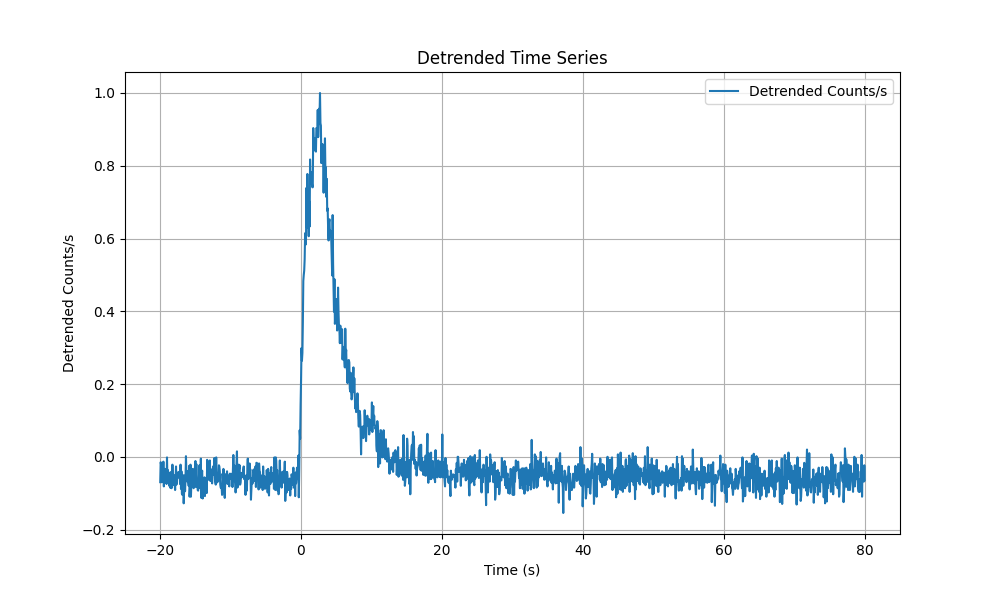
\includegraphics[width=0.7\textwidth]{detrended_time_series.png}
\end{figure}

Then we can do the following analysis for this light curve.

\begin{figure}[ht]
    \centering
    \subfigure[normal][Diagram for ACF]{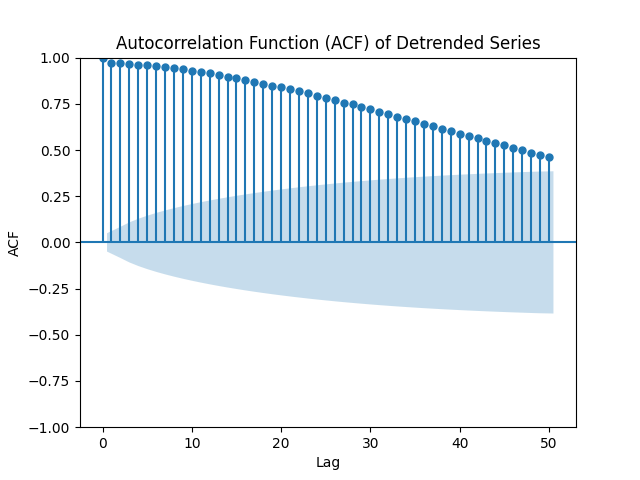
\includegraphics[width=0.4\textwidth]{ACF.png}}
    \subfigure[Diagram for decomposition]{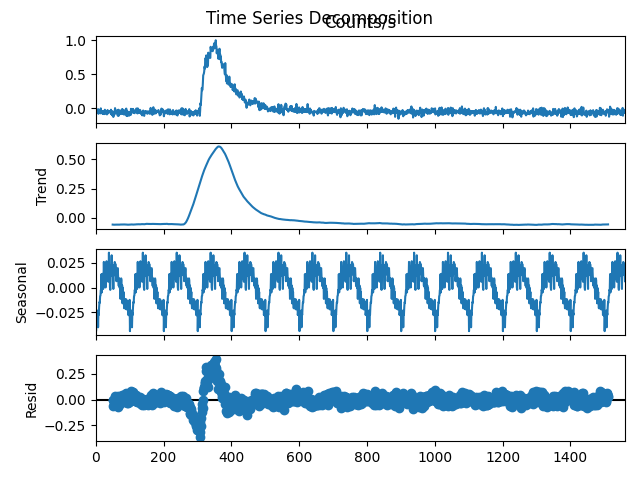
\includegraphics[width=0.4\textwidth]{decomposition.png}}\\
    \subfigure[Diagram for light curve's histogram]{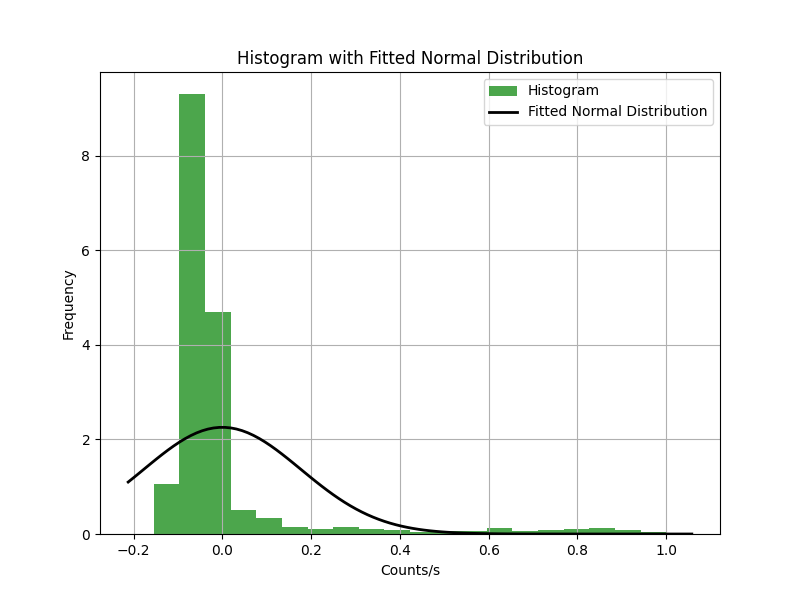
\includegraphics[width=0.4\textwidth]{histogram.png}}
    \subfigure[Diagram for light curve's scatter plot]{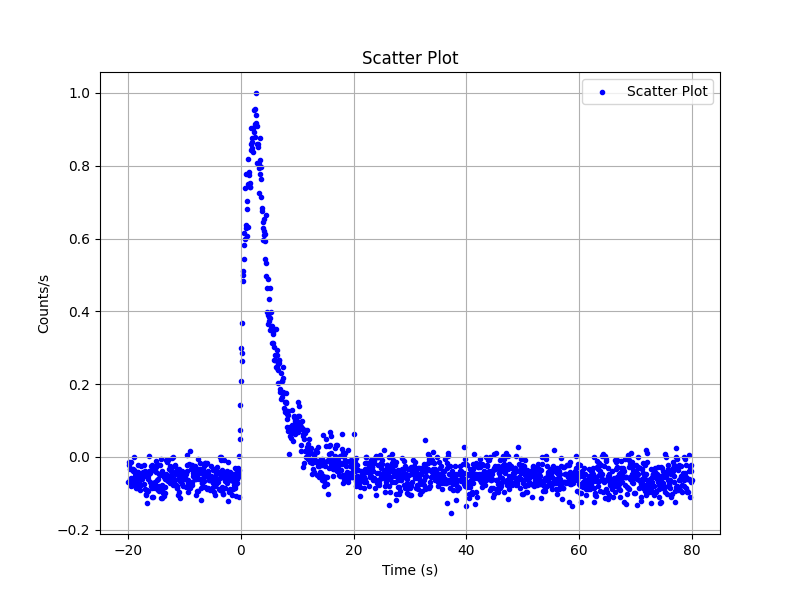
\includegraphics[width=0.4\textwidth]{scatter_plot.png}}\\
    \subfigure[Cumulative plot]{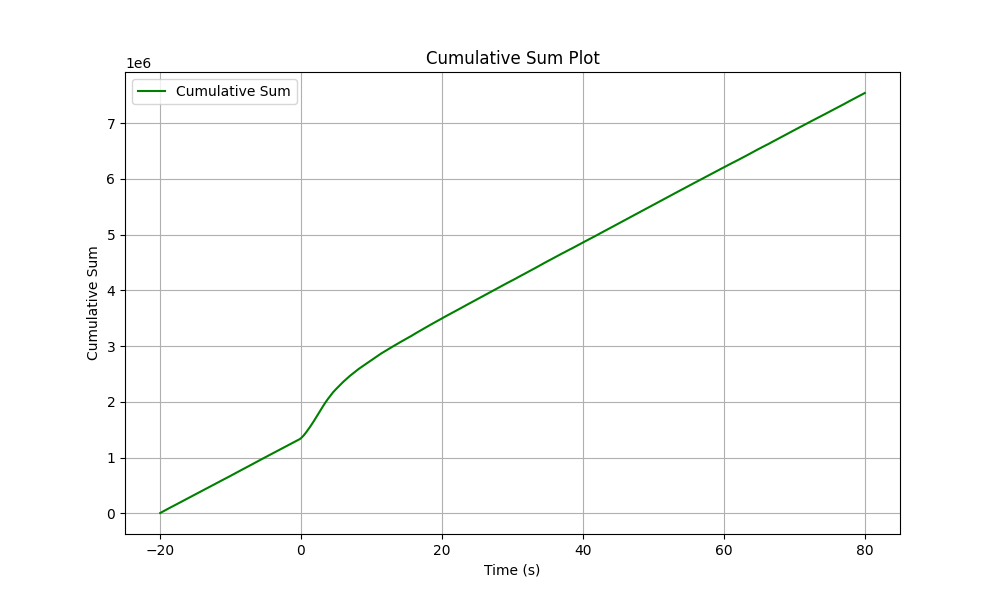
\includegraphics[width=0.4\textwidth]{cumulative.png}}
    \subfigure[Interpolated Plot]{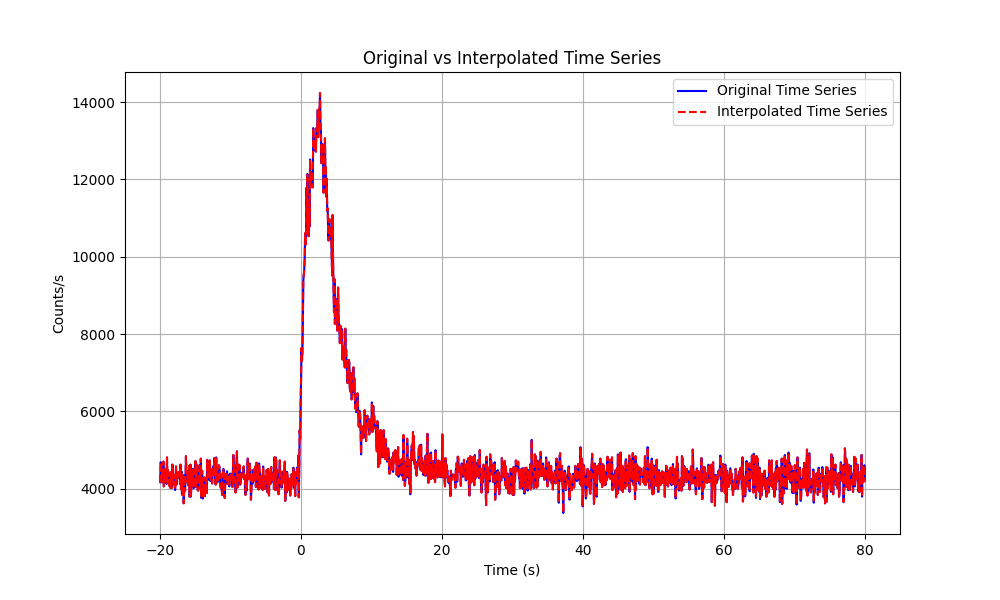
\includegraphics[width=0.4\textwidth]{interpolated.png}}
\end{figure}

\newpage

\section{Appendix File}

\subsection{Log.txt}

\lstinputlisting[caption={log.txt}, label={lst:txt_file}]{log.txt}


\end{document}